% !TeX document-id = {66b2d4b6-7613-4c19-b40c-a50fc00d38ff}
% !TeX program = lualatex
% !BIB program = biber
% Lualatex is important to render TTF fonts; with pdflatex it's just the regular one
% ratio 16:9 -- https://tex.stackexchange.com/questions/14336/

% compile two versions, inspired by https://tex.stackexchange.com/a/1501
% use the script "compile-pdf.sh"
\newif\ifhandout
% if flags.tex does not exist, create an empty file to be able to compile in TeXstudio
\input{flags}

\ifhandout
\documentclass[12pt,aspectratio=169,handout]{beamer}
\else
\documentclass[12pt,aspectratio=169]{beamer}
\fi

% adjust for 16:9
% https://tex.stackexchange.com/questions/354022/modifying-the-margins-of-all-slides-in-beamer
\setbeamersize{text margin left=0.3cm,text margin right=4.5cm} 

%\usepackage{xcolor}

% use Metropolis as the basis theme
\usetheme[subsectionpage=progressbar]{metropolis}
% blocks with background globally
\metroset{block=fill}

% ------- Paderborn specifics ----------
\usepackage{fontspec}
%\setsansfont{karla} % looked bad, too fat
\setsansfont{Segoe UI} % looks OK-ish

% Paderborn color scheme
\definecolor{UPBUltraBlue}{RGB}{0, 37, 170}

\setbeamercolor{frametitle}{bg=white, fg=UPBUltraBlue}

% name in footer
\setbeamertemplate{frame numbering}{Prof.\ Dr.\ Ivan Habernal ~ | ~ \insertframenumber }

% adjust the background to be completely white
\setbeamercolor{background canvas}{bg=white}

% add Paderborn logo at each slide
% actually not -- it's just eating up space
%\addtobeamertemplate{frametitle}{}{%
	%\begin{tikzpicture}[remember picture,overlay]
	%	\node[anchor=north east,yshift=2pt] at (current page.north east) {
\includegraphics[height=0.9cm]{img/UPB_Logo_ENG_coloured_RGB}};
	%\end{tikzpicture}
	%}

% show TOC at every section start
\AtBeginSection{
	\frame{
		\vspace{2em}
		\sectionpage
		\hspace*{2.2em}\begin{minipage}{10cm}
			\tableofcontents[currentsection]
		\end{minipage}
		% we need the logo to show up here as well
		\begin{tikzpicture}[remember picture,overlay]
			\node[anchor=north east,yshift=2pt] at (current page.north east) {
\includegraphics[height=0.9cm]{img/UPB_Logo_ENG_coloured_RGB}};
		\end{tikzpicture}
	}
}
% ------- end of Paderborn specifics ----------


% typeset mathematics on serif
\usefonttheme[onlymath]{serif}

% better bibliography using biber as backend
\usepackage[natbib=true,backend=biber,style=authoryear-icomp,maxbibnames=30,maxcitenames=9,uniquelist=false,giveninits=true,doi=false,url=false,dashed=false,isbn=false]{biblatex}
% shared bibliography
\addbibresource{../nlpwdl-bibliography.bib}
% disable "ibid" for repeated citations
\boolfalse{citetracker}



\usepackage{xspace}


% for derivatives, https://tex.stackexchange.com/a/412442
\usepackage{physics}

\usepackage{tikz}
\usetikzlibrary{matrix, positioning}
\usetikzlibrary{angles,quotes} % for angles
\usetikzlibrary{backgrounds} % background
\usetikzlibrary{decorations.pathreplacing} % curly braces
\usetikzlibrary{calligraphy}
\usetikzlibrary{calc} % for neural nets

% for plotting functions
\usepackage{pgfplots}
\usepgfplotslibrary{dateplot}

% sub-figures
\usepackage{caption}
\usepackage{subcaption}

% book tabs
\usepackage{booktabs}


% argmin, argmax
\usepackage{amsmath}
\DeclareMathOperator*{\argmax}{arg\!\max}
\DeclareMathOperator*{\argmin}{arg\!\min}
% softmax
\DeclareMathOperator*{\softmax}{soft\!\max}

% bold math
\usepackage{bm}

% for \mathclap
\usepackage{mathtools}

% algorithms
\usepackage[noend]{algpseudocode}


% for neurons and layers in tikz
\tikzset{
	neuron/.style={draw, rectangle, inner sep=2pt, minimum width=0.75cm, fill=blue!20},
	param/.style={draw, rectangle, inner sep=2pt, minimum width=0.75cm, fill=green!20},
	constant/.style={draw, rectangle, inner sep=2pt, minimum width=0.75cm, fill=black!15},
	% for citation nodes right top
	ref/.style={anchor = north east, text width=7.8cm, yshift=-1.3cm, xshift=-0.2cm, scale=0.5},
	state/.style={rectangle, inner sep=2pt, minimum width=0.75cm, fill=black!5},
}

% for strike-through text (added in Lecture 06)
\usepackage[normalem]{ulem}

% added in Lecture 7
% RNN
\DeclareMathOperator*{\rnn}{RNN}
% RNN star
\DeclareMathOperator*{\rnnstar}{RNN^{*}}
% bi-RNN
\DeclareMathOperator*{\birnn}{biRNN}


% added in Lecture 9
\usetikzlibrary{fit} % for hightligting by calling "fit"

% algorithms
\usepackage[noend]{algpseudocode}


\title{Natural Language Processing with Deep Learning}
\subtitle{Lecture 9 -- Text classification 5: Introduction to transformers with BERT}
\date{December 8, 2023}
\author{Prof.\ Dr.\ Ivan Habernal}
\institute{Natural Language Processing Group 
	\hfill 
\includegraphics[height=1.4cm]{img/UPB_Logo_ENG_coloured_RGB} \\
	Paderborn University \\
	We focus on Trustworthy Human Language Technologies \hfill \texttt{www.trusthlt.org} }

\begin{document}

\maketitle

\begin{frame}{Motivation}

Problems: Token (word) embeddings -- do not model contextual information

We want contextualized token embeddings

RNN processes left-to-right (or right-to-left)


\end{frame}




\begin{frame}{BERT --- The "NLP gamechanger"}
	
	\begin{columns}
		\begin{column}{0.5\textwidth}
			Best paper award at NAACL 2019
			
			\bigskip
			
			State-of-the-art results on various NLP tasks
			
			\bigskip
			
			Directly applicable to other domains and languages
			
			
		\end{column}
		\begin{column}{0.5\textwidth}
			\vspace{4em}
			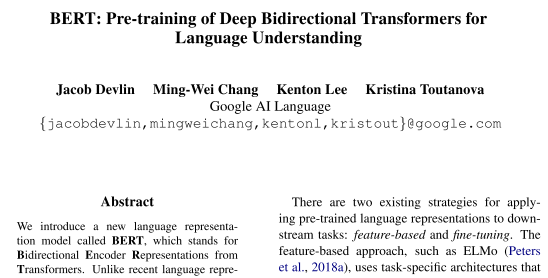
\includegraphics[width=\linewidth]{img/bert-paper01.png}
		\end{column}
	\end{columns}


\begin{tikzpicture}[overlay, remember picture] 
	\node at (current page.north east)[ref] {\fullcite{Devlin.et.al.2019.NAACL} \par};
\end{tikzpicture}


\end{frame}




\section{Neural Machine Translation}

\begin{frame}{Neural machine translation (NMT)}
	Why machine translation here?
	
	BERT builds upon techniques from MT
	
	\begin{columns}
		\begin{column}{0.5\textwidth}
			What is machine translation?
			
			\begin{itemize}
				\item Another popular NLP task
				\item Many large-scale parallel corpora available
			\end{itemize}
			
			
		\end{column}
		\begin{column}{0.4\textwidth}
			\begin{figure}
				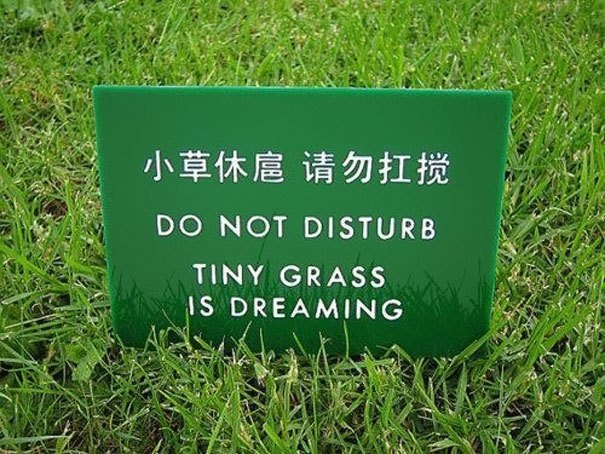
\includegraphics[width=\linewidth]{img/nmt.jpg}
				\caption{MT is a challenging task!}
			\end{figure}	
			
		\end{column}
	\end{columns}
	
	\begin{scriptsize}
		Image source: \url{https://languagelog.ldc.upenn.edu/nll/?p=3978}
	\end{scriptsize}
\end{frame}

\begin{frame}{Recurrent networks for neural MT}
	
	Traditionally \textbf{encoder-decoder} architectures	
	
	\begin{itemize}
		\item One recurrent neural network processes the entire input and generate its dense representation (\textbf{encoder})
		\item Other recurrent network produces one token at the time conditioned on the previous states and generated tokens (\textbf{decoder})
	\end{itemize}
\end{frame}


\begin{frame}{Neural MT: Typical architectures (up to 2016-2017)}
	
	Long short-term memory (LSTM) / GRU networks
	
	
	\begin{figure}
		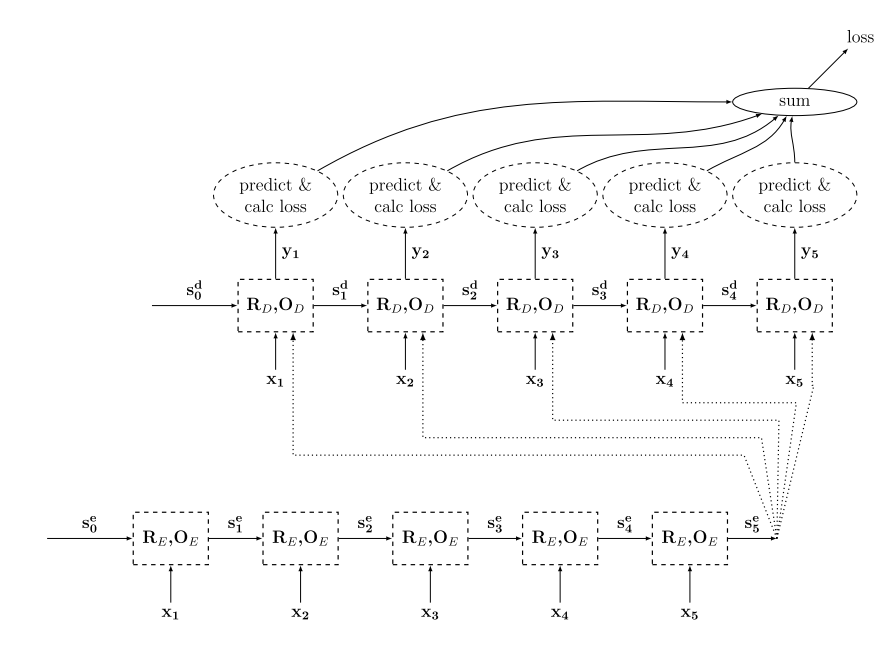
\includegraphics[width=0.65\linewidth]{img/end-dec.png}
		\caption{Encoder-decoder RNN}
	\end{figure}
	
\begin{tikzpicture}[overlay, remember picture] 
	\node at (current page.north east)[ref] {Figure from \fullcite{Goldberg.2016} \par};
\end{tikzpicture}

\end{frame}


\begin{frame}{Bottlenecks of RNN for machine translation?}
	Inherently \textbf{sequential} nature
	
	\begin{itemize}
		\item No parallelization
		\item Big memory footprint (you must "remember" the entire sequence)
		\item Long-range dependencies modeling: Distance plays a role!
	\end{itemize}
	
	...but when the goal is to learn a good representation of the input sequence, why not use...
	
	\begin{itemize}
		\item Convolutional neural networks?
	\end{itemize}
	
\end{frame}

\begin{frame}{Convolutional neural nets (CNN)}
	
	One particular property of CNNs
	
	\begin{itemize}
		\item Modeling dependencies for a \textbf{local context}, but by \textbf{stacking layers}, one exactly controls the context size
	\end{itemize}	
	
	
	\begin{figure}
		
		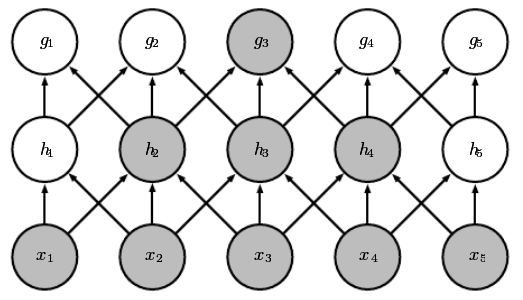
\includegraphics[width=0.5\linewidth]{img/dl-book-cnn.png}	
		\caption{Receptive field of units in deeper layers is larger}
	\end{figure}

\begin{tikzpicture}[overlay, remember picture] 
	\node at (current page.north east)[ref] {Figure from \fullcite{Goodfellow.et.al.2016.book} \par};
\end{tikzpicture}
	
\end{frame}


\begin{frame}{Convolutional neural nets for MT}
	
	CNNs competitive with RNNs for MT\footnote{\citet{Gehring.et.al.2017a.ICML}, Facebook AI Research}
	
	\begin{itemize}
		\item Input tokens as word embeddings (not new) or sub-words (will be explained later)
		\item Fixed-length input? Set-up a maximum length and use \texttt{<PAD>}ding
		\item But positional information of tokens is lost...
	\end{itemize}
	
\begin{tikzpicture}[overlay, remember picture] 
	\node at (current page.north east)[ref] {\fullcite{Gehring.et.al.2017a.ICML} \par};
\end{tikzpicture}
\end{frame}

\begin{frame}{Convolutional neural nets for MT by \citet{Gehring.et.al.2017a.ICML}}
	
	Solution: Positional embeddings
	
	\begin{itemize}
		\item For each input position $n$, train another embedding vector $P_n$: $P_1 = (1.12, -78.6, \dots), P_2, \dots, P_N$
		
		\item Word embeddings and position embeddings are simply summed up for each input token
		
		\item Why? The model knows with which part of the input/output is dealing with
		
		\begin{itemize}
			\item Notice: Removing positional embeddings $\to$ only slightly worse performance
		\end{itemize}
		
		
	\end{itemize}
	
	
	State-of-the-art results and \textbf{9.3--21.3$\times$ faster} than LSTMs on GPU
	
\end{frame}

\section{Attention ``is all you need"}

\begin{frame}{Attention: Modeling dependencies}
	
	Recap: How to model long-range dependencies in input?
	
	\begin{figure}
		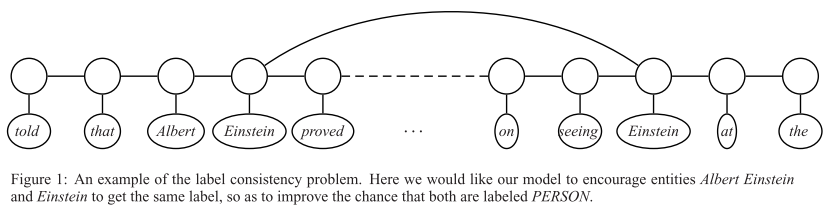
\includegraphics[width=0.95\linewidth]{img/long-deps.png}
	\end{figure}
	
	
	-- RNNs or stacking CNNs
	
	-- \textbf{Self-Attention}: Utilize associations between all input word pairs
	
\begin{tikzpicture}[overlay, remember picture] 
	\node at (current page.north east)[ref] {Figure source: \fullcite{Krishnan.Manning.2006} \par};
\end{tikzpicture}
	
\end{frame}



\begin{frame}{Self-Attention in detail (1)}
	
	
	\begin{figure}
		\scalebox{0.75}{\hspace{-2cm}
			\usetikzlibrary{matrix}
\usetikzlibrary{positioning}
\usetikzlibrary{calc}
\usetikzlibrary{backgrounds}
\usetikzlibrary{fit} % for hightligting by calling "fit"

\tikzset{
	mtx/.style={
		matrix of math nodes,
		left delimiter={[}, right delimiter={]}
	},
	hlt/.style={opacity=0.1, line width=4 mm, line cap=round},
	hltr/.style={opacity=0.5, rounded corners=2pt, inner sep=-1pt}
}

\begin{tikzpicture}

\matrix[mtx, ampersand replacement=\&] (X) at (2,2) {
	\mathrm{The} \\ 
	\mathrm{cat}\\ 
	\mathrm{sat}\\ 
	\mathrm{.} \\
	\mathrm{PAD} \\ 
};

\matrix[mtx,  ampersand replacement=\&, right=5ex of X] (matrixh) { 
   \cdots \& h_1 \&  \cdots \\
   \cdots \& h_2 \&  \cdots \\
   \cdots \& h_3 \&  \cdots \\
   \cdots \& h_4 \&  \cdots \\
   \cdots \& h_5 \&  \cdots \\
};

\matrix[mtx, ampersand replacement=\&, nodes={anchor=west}, right=of matrixh] (matrixhtrans) {
   \vdots \& \vdots \&  \vdots \& \vdots \& \vdots \\
   h_1 \& h_2 \& h_3 \& h_4 \& h_5 \\
   \vdots \& \vdots \&  \vdots \& \vdots \& \vdots \\
};

\matrix[mtx, ampersand replacement=\&, nodes={anchor=west}, right=of matrixhtrans] (raw) {
   11 \& 12 \& 13 \& 14 \& 15 \\
   21 \& \ddots \& \& \& \vdots  \\
   31 \&  \& \ddots \&  \& \vdots \\
   41 \&  \&  \& \ddots \& \vdots \\
   51 \&  \cdots \& \cdots  \& \cdots  \& 55 \\
};

%\draw[-stealth, color=red] (X-1-1.south west) -| (beta-6-1.south west);

%\node at ($(X.east) !0.5! (matrixh.west)$) {$*$};
\node at ($(matrixh.east)!0.5!(matrixhtrans.west)$) {$\times$};%
\node at ($(matrixhtrans.east)!0.5!(raw.west)$) {$=$};%


\begin{scope}[on background layer]
%\node[hltr, fill=gray, fit=(beta-1-1)] {};
%\node[hltr, fill=red, fit=(beta-2-1)(beta-3-1)] {};
%\node[hltr, fill=green, fit=(beta-4-1)(beta-6-1)] {};
%\node[hltr, fill=gray, fit=(X-1-1)(X-12-1)] {};
%\node[hltr, fill=orange, fit=(filterg-1-1)(filterg-3-3)] {};
\foreach \in in {1,2,3,4,5} {
\node[hltr, fill=green, fit=(matrixh-\in-1)(matrixh-\in-3)] {};
}
\foreach \in in {1,2,3,4,5} {
\node[hltr, fill=green, fit=(matrixhtrans-1-\in)(matrixhtrans-3-\in)] {};
}
%\node[hltr, fill=orange, fit=(mu-1-1)(mu-1-1)] {};
\node[hltr, fill=lightgray, fit=(raw-1-1)(raw-5-5)] {};
\end{scope}


\foreach \in in {1,2,3,4,5} {
	\draw[->, lightgray, thick] (X-\in-1) to[out = 0, in = 180] (matrixh-\in-1);
}



\begin{scope}[every node/.style={align=center,text width=3cm}]
\node[below=0.2cm of X] (inputdsc) {\scriptsize Input tokens};
\node[below=0.2cm of matrixh] (convdesc) {\scriptsize Matrix $H$ \\ (latent representation)};
\node[below=0.5cm of matrixhtrans] (outdesc) {\scriptsize Matrix $H$ transposed};
\node[below=0.5cm of raw] (outdesc) {\scriptsize Dot product (raw associations) \\  Scale each row by $\sqrt{|h|}$};
%\node[above=0cm of hidden] (hiddendsc) {\scriptsize Hidden layer};
%\node[above=0cm of output] (outputdsc) {\scriptsize Output};


\end{scope}


\end{tikzpicture}
		}
	\end{figure}
	
\end{frame}

\begin{frame}{Self-Attention in detail (2)}
	
	
	\begin{figure}
		\scalebox{0.75}{\hspace{-2cm}
			\usetikzlibrary{matrix}
\usetikzlibrary{positioning}
\usetikzlibrary{calc}
\usetikzlibrary{backgrounds}
\usetikzlibrary{fit} % for hightligting by calling "fit"

\tikzset{
	mtx/.style={
		matrix of math nodes,
		left delimiter={[}, right delimiter={]}
	},
	hlt/.style={opacity=0.1, line width=4 mm, line cap=round},
	hltr/.style={opacity=0.5, rounded corners=2pt, inner sep=-1pt}
}

\begin{tikzpicture}

\matrix[mtx, ampersand replacement=\&] (X) at (2,2) {
	\mathrm{The} \\ 
	\mathrm{cat}\\ 
	\mathrm{sat}\\ 
	\mathrm{.} \\
	\mathrm{PAD} \\ 
};


\matrix[mtx, ampersand replacement=\&, nodes={anchor=west}, right=of X] (raw) {
   11 \& 12 \& 13 \& 14 \& 15 \\
   21 \& \ddots \& \& \& \vdots  \\
   31 \&  \& \ddots \&  \& \vdots \\
   41 \&  \&  \& \ddots \& \vdots \\
   51 \&  \cdots \& \cdots  \& \cdots  \& 55 \\
};

\matrix[mtx, ampersand replacement=\&, nodes={anchor=west}, right=4cm of raw] (probabilistic) {
   11 \& 12 \& 13 \& 14 \& 15 \\
   21 \& \ddots \& \& \& \dots  \\
   31 \&  \& \ddots \&  \& \dots \\
   41 \&  \&  \& \ddots \& \dots \\
   51 \&  \cdots \& \cdots  \& \cdots  \& 55 \\
};

%\draw[-stealth, color=red] (X-1-1.south west) -| (beta-6-1.south west);

%\node at ($(X.east) !0.5! (matrixh.west)$) {$*$};
%\node at ($(matrixh.east)!0.5!(matrixhtrans.west)$) {$\times$};%
\node at ($(raw.north)!0.5!(probabilistic.north)$) {\scriptsize Softmax (per row)};%


\begin{scope}[on background layer]
%\node[hltr, fill=gray, fit=(beta-1-1)] {};
%\node[hltr, fill=red, fit=(beta-2-1)(beta-3-1)] {};
%\node[hltr, fill=green, fit=(beta-4-1)(beta-6-1)] {};
%\node[hltr, fill=gray, fit=(X-1-1)(X-12-1)] {};
%\node[hltr, fill=orange, fit=(filterg-1-1)(filterg-3-3)] {};

%\node[hltr, fill=orange, fit=(mu-1-1)(mu-1-1)] {};
\node[hltr, fill=lightgray, fit=(raw-1-1)(raw-5-5)] {};
\foreach \in in {1,2,3,4,5} {
	\node[hltr, fill=yellow, fit=(probabilistic-\in-1)(probabilistic-\in-5)] {};
}
\end{scope}


\foreach \in in {1,2,3,4,5} {
	\draw[->, lightgray, thick, dashed] (X-\in-1) to[out = 0, in = 180] (raw-\in-1);
}

\foreach \in in {1,2,3,4,5} {
	\draw[->, lightgray, thick] (raw-\in-5) to[out = 0, in = 180] (probabilistic-\in-1);
}


\begin{scope}[every node/.style={align=center,text width=3cm}]
\node[below=0.2cm of X] (inputdsc) {\scriptsize Input tokens};
\node[below=0cm of raw] (outdesc) {\scriptsize Dot product (raw associations)};
\node[below=0cm of probabilistic] (outdesc) {\scriptsize Normalized associations};
%\node[above=0cm of hidden] (hiddendsc) {\scriptsize Hidden layer};
%\node[above=0cm of output] (outputdsc) {\scriptsize Output};


\end{scope}


\end{tikzpicture}
		}
	\end{figure}
	
	\begin{itemize}
		\item 	Each row corresponds to an input token
		
		\item Each row sums up to 1
		
		\item Each cell shows the "association strength" with all other tokens
		
	\end{itemize}
	
	
\end{frame}



\begin{frame}{Self-Attention in detail (3)}
	
	
	\begin{figure}
		\scalebox{0.75}{\hspace{-2cm}
			\usetikzlibrary{matrix}
\usetikzlibrary{positioning}
\usetikzlibrary{calc}
\usetikzlibrary{backgrounds}
\usetikzlibrary{fit} % for hightligting by calling "fit"

\tikzset{
	mtx/.style={
		matrix of math nodes,
		left delimiter={[}, right delimiter={]}
	},
	hlt/.style={opacity=0.1, line width=4 mm, line cap=round},
	hltr/.style={opacity=0.5, rounded corners=2pt, inner sep=-1pt}
}

\begin{tikzpicture}

\matrix[mtx, ampersand replacement=\&] (X) at (2,2) {
	\mathrm{The} \\ 
	\mathrm{cat}\\ 
	\mathrm{sat}\\ 
	\mathrm{.} \\
	\mathrm{PAD} \\ 
};




\matrix[mtx, ampersand replacement=\&, nodes={anchor=west}, right=of X] (probabilistic) {
   11 \& 12 \& 13 \& 14 \& 15 \\
   21 \& \ddots \& \& \& \dots  \\
   31 \&  \& \ddots \&  \& \dots \\
   41 \&  \&  \& \ddots \& \dots \\
   51 \&  \cdots \& \cdots  \& \cdots  \& 55 \\
};

\matrix[mtx,  ampersand replacement=\&, right=5ex of probabilistic] (matrixh) { 
   \cdots \& h_1 \&  \cdots \\
   \cdots \& h_2 \&  \cdots \\
   \cdots \& h_3 \&  \cdots \\
   \cdots \& h_4 \&  \cdots \\
   \cdots \& h_5 \&  \cdots \\
};

\matrix[mtx,  ampersand replacement=\&, right=5ex of matrixh] (selfattention) { 
   \cdots \& h_1 \&  \cdots \\
   \cdots \& h_2 \&  \cdots \\
   \cdots \& h_3 \&  \cdots \\
   \cdots \& h_4 \&  \cdots \\
   \cdots \& h_5 \&  \cdots \\
};

%\draw[-stealth, color=red] (X-1-1.south west) -| (beta-6-1.south west);

%\node at ($(X.east) !0.5! (matrixh.west)$) {$*$};
\node at ($(probabilistic.east)!0.5!(matrixh.west)$) {$\times$};%
\node at ($(matrixh.east)!0.5!(selfattention.west)$) {$=$};%
%\node at ($(raw.north)!0.5!(probabilistic.north)$) {Softmax (per row)};%


\begin{scope}[on background layer]
%\node[hltr, fill=gray, fit=(beta-1-1)] {};
%\node[hltr, fill=red, fit=(beta-2-1)(beta-3-1)] {};
%\node[hltr, fill=green, fit=(beta-4-1)(beta-6-1)] {};
%\node[hltr, fill=gray, fit=(X-1-1)(X-12-1)] {};
%\node[hltr, fill=orange, fit=(filterg-1-1)(filterg-3-3)] {};

%\node[hltr, fill=orange, fit=(mu-1-1)(mu-1-1)] {};
%\node[hltr, fill=lightgray, fit=(raw-1-1)(raw-5-5)] {};

\foreach \in in {1,2,3,4,5} {
	\node[hltr, fill=green, fit=(matrixh-\in-1)(matrixh-\in-3)] {};
}

\foreach \in in {1,2,3,4,5} {
	\node[hltr, fill=yellow, fit=(probabilistic-\in-1)(probabilistic-\in-5)] {};
}

\foreach \in in {1,2,3,4,5} {
	\node[hltr, fill=orange, fit=(selfattention-\in-1)(selfattention-\in-3)] {};
}
\end{scope}


% \foreach \in in {1,2,3,4,5} {
% 	\draw[->, lightgray, thick, dashed] (X-\in-1) to[out = 0, in = 180] (raw-\in-1);
% }

% \foreach \in in {1,2,3,4,5} {
% 	\draw[->, lightgray, thick] (X-\in-5) to[out = 0, in = 180] (probabilistic-\in-1);
% }

\foreach \in in {1,2,3,4,5} {
	\draw[->, lightgray, thick, dashed] (X-\in-1) to[out = 0, in = 180] (probabilistic-\in-1);
}


\begin{scope}[every node/.style={align=center,text width=3cm}]
\node[below=0.2cm of X] (inputdsc) {\scriptsize Input tokens};
\node[below=0.2cm of matrixh] (convdesc) {\scriptsize Matrix $H$};
% \node[below=0.5cm of raw] (outdesc) {\scriptsize Dot product (raw associations)};
\node[below=0cm of probabilistic] (outdesc) {\scriptsize Normalized associations};
\node[below=0cm of selfattention] (outdesc) {\scriptsize Self-attention};
%\node[above=0cm of hidden] (hiddendsc) {\scriptsize Hidden layer};
%\node[above=0cm of output] (outputdsc) {\scriptsize Output};


\end{scope}


\end{tikzpicture}
		}
	\end{figure}
	
	
	Each position in the latent representation of a token is weighted by the association strength with other tokens
	
	
\end{frame}


\begin{frame}{Self-Attention in detail (4)}
	
	
	\begin{figure}
		\scalebox{0.75}{\hspace{-2cm}
			\usetikzlibrary{matrix}
\usetikzlibrary{positioning}
\usetikzlibrary{calc}
\usetikzlibrary{backgrounds}
\usetikzlibrary{fit} % for hightligting by calling "fit"

\tikzset{
	mtx/.style={
		matrix of math nodes,
		left delimiter={[}, right delimiter={]}
	},
	hlt/.style={opacity=0.1, line width=4 mm, line cap=round},
	hltr/.style={opacity=0.5, rounded corners=2pt, inner sep=-1pt}
}

\begin{tikzpicture}

\matrix[mtx,  ampersand replacement=\& ] (selfattention) at (2,2) { 
   \cdots \& h_1 \&  \cdots \\
   \cdots \& h_2 \&  \cdots \\
   \cdots \& h_3 \&  \cdots \\
   \cdots \& h_4 \&  \cdots \\
   \cdots \& h_5 \&  \cdots \\
};


\matrix[mtx,  ampersand replacement=\&, right=5ex of selfattention] (matrixh) { 
   \cdots \& h_1 \&  \cdots \\
   \cdots \& h_2 \&  \cdots \\
   \cdots \& h_3 \&  \cdots \\
   \cdots \& h_4 \&  \cdots \\
   \cdots \& h_5 \&  \cdots \\
};

\matrix[mtx,  ampersand replacement=\&, right=5ex of matrixh] (residual) { 
   \cdots \& h_1 \&  \cdots \\
   \cdots \& h_2 \&  \cdots \\
   \cdots \& h_3 \&  \cdots \\
   \cdots \& h_4 \&  \cdots \\
   \cdots \& h_5 \&  \cdots \\
};

%\draw[-stealth, color=red] (X-1-1.south west) -| (beta-6-1.south west);

%\node at ($(X.east) !0.5! (matrixh.west)$) {$*$};
% \node at ($(probabilistic.east)!0.5!(matrixh.west)$) {$\times$};%
\node at ($(selfattention.east)!0.5!(matrixh.west)$) {$+$};%
\node at ($(matrixh.east)!0.5!(residual.west)$) {$=$};%
%\node at ($(raw.north)!0.5!(probabilistic.north)$) {Softmax (per row)};%


\begin{scope}[on background layer]
%\node[hltr, fill=gray, fit=(beta-1-1)] {};
%\node[hltr, fill=red, fit=(beta-2-1)(beta-3-1)] {};
%\node[hltr, fill=green, fit=(beta-4-1)(beta-6-1)] {};
%\node[hltr, fill=gray, fit=(X-1-1)(X-12-1)] {};
%\node[hltr, fill=orange, fit=(filterg-1-1)(filterg-3-3)] {};

%\node[hltr, fill=orange, fit=(mu-1-1)(mu-1-1)] {};
%\node[hltr, fill=lightgray, fit=(raw-1-1)(raw-5-5)] {};

\foreach \in in {1,2,3,4,5} {
\node[hltr, fill=green, fit=(matrixh-\in-1)(matrixh-\in-3)] {};
}

\foreach \in in {1,2,3,4,5} {
	\node[hltr, fill=orange, fit=(selfattention-\in-1)(selfattention-\in-3)] {};
}

\foreach \in in {1,2,3,4,5} {
	\node[hltr, fill=blue!20, fit=(residual-\in-1)(residual-\in-3)] {};
}
\end{scope}


% \foreach \in in {1,2,3,4,5} {
% 	\draw[->, lightgray, thick, dashed] (X-\in-1) to[out = 0, in = 180] (raw-\in-1);
% }

% \foreach \in in {1,2,3,4,5} {
% 	\draw[->, lightgray, thick] (X-\in-5) to[out = 0, in = 180] (probabilistic-\in-1);
% }

% \foreach \in in {1,2,3,4,5} {
% 	\draw[->, lightgray, thick, dashed] (X-\in-1) to[out = 0, in = 180] (probabilistic-\in-1);
% }


\begin{scope}[every node/.style={align=center,text width=3cm}]
% \node[below=0.5cm of raw] (outdesc) {\scriptsize Dot product (raw associations)};
\node[below=0cm of matrixh] (convdesc) {\scriptsize Matrix $H$};
\node[below=0cm of selfattention] (outdesc2) {\scriptsize Self-attention};
\node[below=0cm of residual] (outdesc3) {\scriptsize "Residual connections"};
%\node[above=0cm of hidden] (hiddendsc) {\scriptsize Hidden layer};
%\node[above=0cm of output] (outputdsc) {\scriptsize Output};


\end{scope}


\end{tikzpicture}
		}
	\end{figure}
	
\end{frame}



\begin{frame}{Self-Attention in detail: Head}
	
	
	\begin{figure}
		\scalebox{0.75}{\hspace{-1.5cm}
			\usetikzlibrary{matrix}
\usetikzlibrary{positioning}
\usetikzlibrary{calc}
\usetikzlibrary{backgrounds}
\usetikzlibrary{fit} % for hightligting by calling "fit"

\tikzset{
	mtx/.style={
		matrix of math nodes,
		left delimiter={[}, right delimiter={]}
	},
	hlt/.style={opacity=0.1, line width=4 mm, line cap=round},
	hltr/.style={opacity=0.5, rounded corners=2pt, inner sep=-1pt}
}

\begin{tikzpicture}

\matrix[mtx, ampersand replacement=\&] (X) at (0,0) {
	\mathrm{The} \\ 
	\mathrm{cat}\\ 
	\mathrm{sat}\\ 
	\mathrm{.} \\
	\mathrm{PAD} \\ 
};

\matrix[mtx,  ampersand replacement=\&, right=of X ] (selfattention) { 
   \cdots \& h_1 \&  \cdots \\
   \cdots \& h_2 \&  \cdots \\
   \cdots \& h_3 \&  \cdots \\
   \cdots \& h_4 \&  \cdots \\
   \cdots \& h_5 \&  \cdots \\
};


\matrix[mtx,  ampersand replacement=\&, right=5ex of selfattention] (residual) { 
   \cdots \& h_1 \&  \cdots \\
   \cdots \& h_2 \&  \cdots \\
   \cdots \& h_3 \&  \cdots \\
   \cdots \& h_4 \&  \cdots \\
   \cdots \& h_5 \&  \cdots \\
};

\matrix[mtx,  ampersand replacement=\&, right=18ex of residual] (head) { 
   \cdots \& h_1 \&  \cdots \\
   \cdots \& h_2 \&  \cdots \\
   \cdots \& h_3 \&  \cdots \\
   \cdots \& h_4 \&  \cdots \\
   \cdots \& h_5 \&  \cdots \\
};

%\draw[-stealth, color=red] (X-1-1.south west) -| (beta-6-1.south west);

%\node at ($(X.east) !0.5! (matrixh.west)$) {$*$};
% \node at ($(probabilistic.east)!0.5!(matrixh.west)$) {$\times$};%
% \node at ($(selfattention.east)!0.5!(matrixh.west)$) {$+$};%
\node at ($(residual.north)!0.5!(head.north)$) {Further OPs};%




\begin{scope}[on background layer]
%\node[hltr, fill=gray, fit=(beta-1-1)] {};
%\node[hltr, fill=red, fit=(beta-2-1)(beta-3-1)] {};
%\node[hltr, fill=green, fit=(beta-4-1)(beta-6-1)] {};
%\node[hltr, fill=gray, fit=(X-1-1)(X-12-1)] {};
%\node[hltr, fill=orange, fit=(filterg-1-1)(filterg-3-3)] {};

%\node[hltr, fill=orange, fit=(mu-1-1)(mu-1-1)] {};
%\node[hltr, fill=lightgray, fit=(raw-1-1)(raw-5-5)] {};


\foreach \in in {1,2,3,4,5} {
	\node[hltr, fill=orange, fit=(selfattention-\in-1)(selfattention-\in-3)] {};
}

\foreach \in in {1,2,3,4,5} {
	\node[hltr, fill=blue!20, fit=(residual-\in-1)(residual-\in-3)] {};
}

\foreach \in in {1,2,3,4,5} {
	\node[hltr, fill=blue!60, fit=(head-\in-1)(head-\in-3)] {};
}

\end{scope}


% \foreach \in in {1,2,3,4,5} {
% 	\draw[->, lightgray, thick, dashed] (X-\in-1) to[out = 0, in = 180] (raw-\in-1);
% }

% \foreach \in in {1,2,3,4,5} {
% 	\draw[->, lightgray, thick] (X-\in-5) to[out = 0, in = 180] (probabilistic-\in-1);
% }

% \foreach \in in {1,2,3,4,5} {
% 	\draw[->, lightgray, thick, dashed] (X-\in-1) to[out = 0, in = 180] (probabilistic-\in-1);
% }

\foreach \in in {1,2,3,4,5} {
	\draw[->, lightgray, thick, dashed] (X-\in-1) to[out = 0, in = 180] (selfattention-\in-1);
}

\foreach \in in {1,2,3,4,5} {
	\draw[->, lightgray, thick, dashed] (selfattention-\in-3) to[out = 0, in = 180] (residual-\in-1);
}

\foreach \in in {1,2,3,4,5} {
	\draw[->, lightgray, thick, dashed] (residual-\in-3) to[out = 0, in = 180] (head-\in-1);
}

\begin{scope}[every node/.style={align=center,text width=3cm}]
% \node[below=0.5cm of raw] (outdesc) {\scriptsize Dot product (raw associations)};
\node[below=0cm of selfattention] (outdesc2) {\scriptsize Self-attention};
\node[below=0cm of residual] (outdesc3) {\scriptsize "Residual connections"};
\node[below=0cm of head] (outdesc3) {\scriptsize Attention "head" output};
%\node[above=0cm of hidden] (hiddendsc) {\scriptsize Hidden layer};
%\node[above=0cm of output] (outputdsc) {\scriptsize Output};


\end{scope}


\end{tikzpicture}
		}
	\end{figure}
	
	Further operations
	
	\begin{itemize}
		\item Layer normalization
		\item Feed-forward layer with ReLU
		\item Another residual connection and layer normalization
	\end{itemize}
	
\end{frame}


\begin{frame}{Self-attention: More subtleties}
	
	\begin{itemize}
		\item Run N attention "heads" in parallel and concatenate
		\item Stack on top of each other M-times
	\end{itemize}
	
	
	Why self-attention?
	
	\begin{itemize}
		\item Self-attention layer connects all positions with a constant number of sequentially executed operations
		\item Recurrent layer requires O(n) sequential operations
		\item Self-attention layers are \textbf{fast}
	\end{itemize}
	
	\begin{footnotesize}
		\fullcite{Vaswani.et.al.2017}
	\end{footnotesize}
	
	
\end{frame}


\section{Multi-task learning}


\begin{frame}{Multi-task Learning}
	
	\begin{columns}
		\begin{column}{0.5\linewidth}
			Approach to inductive transfer that improves generalization
			
			\bigskip	
			
			By learning tasks in parallel while using a shared representation
			
		\end{column}
		\begin{column}{0.5\linewidth}
			\begin{figure}
				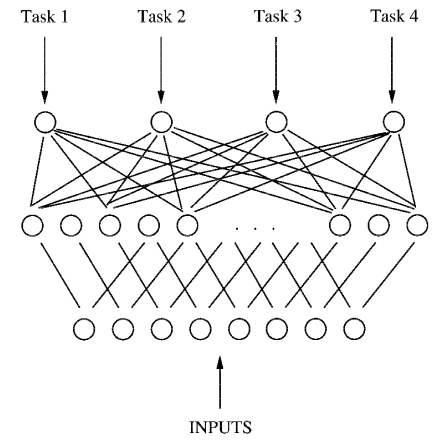
\includegraphics[width=\linewidth]{img/multitask.png}	
			\end{figure}
			
		\end{column}
	\end{columns}
	
	\bigskip
	
	\begin{footnotesize}
		\fullcite{Caruana.1997}
	\end{footnotesize}
	
	
\end{frame}



\begin{frame}{Multi-task learning in NLP}
	
	\begin{columns}
		\begin{column}{0.5\linewidth}
			
			\begin{small}
				\emph{"In case we suspect the existence of a hierarchy between the different tasks, we show that it is worth-while to incorporate this knowledge in the MTL architecture’s design, by making lower level tasks affect the lower levels of the representation." }
			\end{small}			
		\end{column}
		\begin{column}{0.5\linewidth}
			
			\begin{figure}
				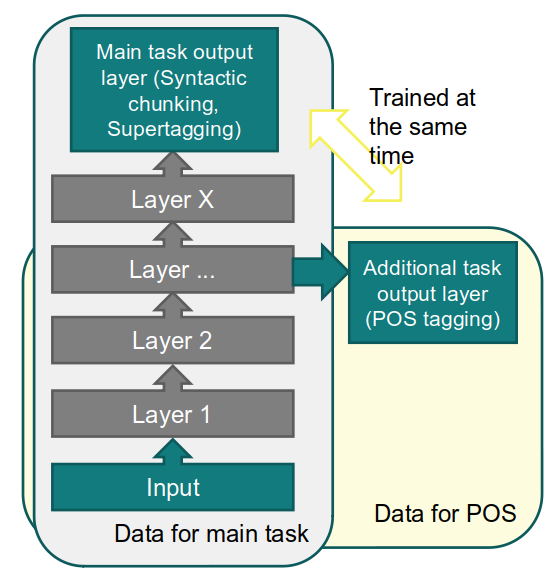
\includegraphics[width=\linewidth]{img/multitask-nlp.png}
			\end{figure}
		\end{column}
	\end{columns}
	
	\bigskip
	
	\begin{footnotesize}
		\fullcite{Sogaard.Goldberg.2016}
	\end{footnotesize}
	
\end{frame}


\begin{frame}{Learn a sentence representation on a different task}
	
	\begin{figure}
		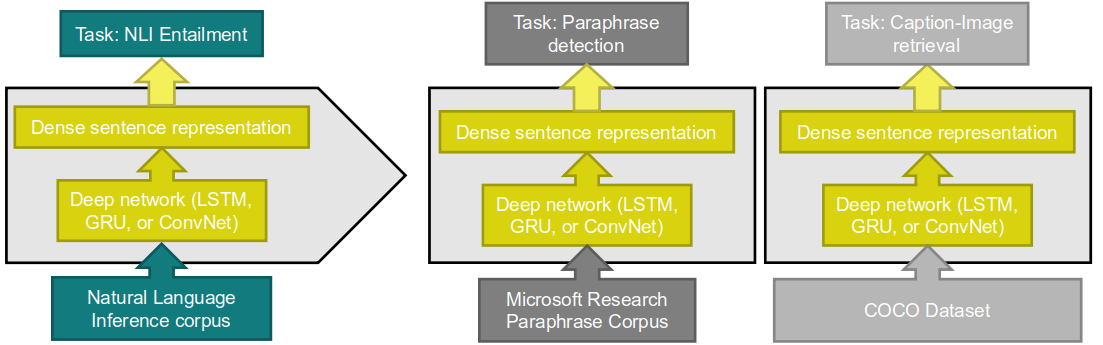
\includegraphics[width=0.9\linewidth]{img/transfer.png}
	\end{figure}
	
	\begin{small}
		\emph{"Models learned on NLI can perform better than models trained in unsupervised conditions or on other supervised tasks."}\footnote{\fullcite{Conneau.et.al.2017.EMNLP}}
	\end{small}
	
	
\end{frame}


\section{BERT}


\begin{frame}{BERT: Very abstract view}
	
	\begin{figure}
		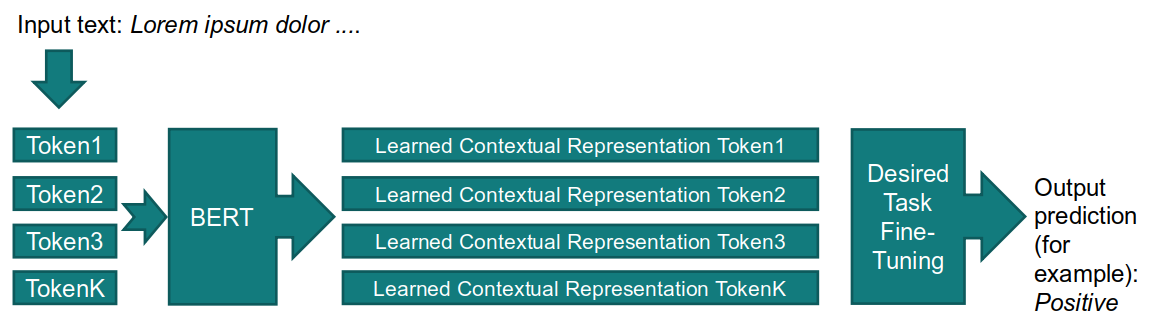
\includegraphics[width=\linewidth]{img/bert1.png}
	\end{figure}	
	
\end{frame}


\begin{frame}{BERT: The transformer encoder}
	
	\begin{columns}
		\begin{column}{0.6\linewidth}
			\begin{itemize}
				\item Multiple parallel attention "heads” (16 heads)
				\item With residual connections
				\item With layer normalization
				\item Stacked on top of each other (24-times)
				\item 310,000,000 trainable parameters
			\end{itemize}
		\end{column}
		\begin{column}{0.3\linewidth}
			\begin{figure}
				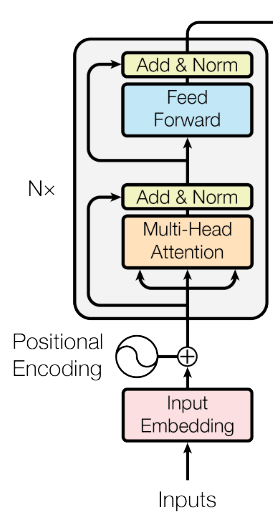
\includegraphics[width=\linewidth]{img/transformer.png}
			\end{figure}
		\end{column}
	\end{columns}
	
\end{frame}


\begin{frame}{Some details (Notation)}
	
	Simplify the set notation
	
	$\{1, 2, \ldots, N\}$ is a set of integers $1, 2, \ldots, N - 1, N$
	
	simplify to $[N]$
	
	For example $t \in [N] \equiv t \in \{1, 2, \ldots, N\}$
	
	
	\begin{tikzpicture}[overlay, remember picture] 
		\node at (current page.north east)[ref] {Notation and formal description of algorithms adopted from \fullcite{Phuong.Hutter.2022} Note that they use column-vector notation while here (and in all lectures) we use row-vector notation. \par};
	\end{tikzpicture}
	
\end{frame}

\begin{frame}{Basic single-query attention}
	
	\begin{minipage}[t][10cm][t]{15cm}
		
		Input: $\bm{e} \in \mathbb{R}^{d_\text{in}}$, vector representation of the current token
		
		Input: $\bm{e}_t \in \mathbb{R}^{d_\text{in}}$, vector representations of the context tokens $t \in [T]$
		
		Output: $\bm{\tilde v} \in \mathbb{R}^{d_\text{out}}$, vector representation of the token and context combined
		
		Params: $\bm{W_q}, \bm{W_k} \in \mathbb{R}^{d_\text{in} \times d_\text{attn}}$, $\bm{b_q}, \bm{b_k} \in \mathbb{R}^{d_\text{attn}}$, the query and key linear projections
		
		$\bm{W_v} \in \mathbb{R}^{d_\text{in} \times d_\text{out}}$, $ \bm{b_v} \in \mathbb{R}^{d_\text{out}}$, the value linear projection
		
		\begin{algorithmic}[1]
			\Function{Basic single-query attention}{}
			%\KwIn{}
			%\KwOut{$\v{\tilde v}∈ℝ^{d_\t{out}}$, vector representation of the token and context combined.}
			%\KwParam{$\m{W_q}, \m{W_k}∈ℝ^{d_\t{attn}×d_\t{in}}$, $ \v{b_q}, \v{b_k}∈ℝ^{d_\t{attn}}$, the query and key linear projections.}
			%\KwParam{$\m{W_v}∈ℝ^{d_\t{out}×d_\t{in}}$, $ \v{b_v}∈ℝ^{d_\t{out}}$, the value linear projection.}
			\State $\bm{q} \gets \bm{e} \bm{W_q} + \bm{b_q}$
			\Comment{Query linear projection}
			\For{$t \in [T]$}
			\State $\bm{k_t} \gets \bm{e_t} \bm{W_k} + \bm{b_k}$
			\Comment{Key linear projection}
			\State $\alpha_{t} = \frac{
				\exp(\bm{q} \cdot \bm{k_t} / \sqrt{d_{\text{attn}}})
			}{
				\sum_{u = 1}^{T}\exp(\bm{q} \cdot \bm{k_u} / \sqrt{d_{\text{attn}}})
			}$
			\Comment{Softmax over scaled dot products ($\alpha_{t} \in \mathbb{R}$)}
			\State $\bm{v_t} \gets \bm{e_t} \bm{W_v} + \bm{b_v}$
			\Comment{Value linear projection}
			\EndFor
			\State \Return $\bm{\tilde v} = \sum_{t=1}^T \alpha_t \bm{v}_t$
			\EndFunction
		\end{algorithmic}
		
	\end{minipage}
\end{frame}



\begin{frame}{Some details}
	
	Concatenate matrices of the same dimensions along rows
	$$\bm{Y} = [\bm{X}^1 ; \bm{X}^2 ; \ldots ; \bm{X}^H]
	\qquad
	\bm{X}^i \in \mathbb{R}^{m \times n}
	\qquad
	\bm{Y} \in \mathbb{R}^{m \times H \cdot n}$$
	
	\begin{block}{Example}
		\begin{small}
			$$
			\bm{A} =
			\begin{pmatrix}
				1 & 2 \\
				3 & 4 \\
				5 & 6
			\end{pmatrix}
			,
			\bm{B} =
			\begin{pmatrix}
				11 & 12 \\
				13 & 14 \\
				15 & 16
			\end{pmatrix}
			\quad
			\bm{Y} = [\bm{A} ; \bm{B} ] =
			\begin{pmatrix}
				1 & 2 & 11 & 12 \\
				3 & 4 & 13 & 14 \\
				5 & 6 & 15 & 16
			\end{pmatrix}
			$$
		\end{small}
	\end{block}
	
	
\end{frame}



\begin{frame}{Some details}
	
	How to add a single vector $\bm{b}$ to each row in a matrix $\bm{W}$ ($\bm{W} \in \mathbb{R}^{m \times n}, \bm{b} \in \mathbb{R}^{n}$)
	
	We want $\bm{Z} = \bm{X} +_{\text{(rows)}} \bm{b}$
	
	Let $\bm{1}^{m} = (1, 1, \ldots, 1_m)$, then $\bm{Z} = \bm{X} +_{\text{(rows)}} \bm{b} = \bm{X} +  (\bm{b}^\top  \bm{1}^{m})^\top$
	
	\begin{block}{Example}
		\begin{scriptsize}
			$$
			\bm{X} =
			\begin{pmatrix}
				1 & 2 \\
				3 & 4 \\
				5 & 6
			\end{pmatrix}
			,
			\bm{b} = \begin{pmatrix}10 & 20\end{pmatrix}
			$$
			
			$$
			\bm{b}^\top \bm{1}^m = \begin{pmatrix}10 \\ 20\end{pmatrix}
			\begin{pmatrix}1 & 1 & 1\end{pmatrix} =
			\begin{pmatrix}10 & 10 & 10 \\ 20 & 20 & 20 \end{pmatrix}
			\qquad
			(\bm{b}^\top \bm{1}^m)^\top = 
			\begin{pmatrix} 10 & 20 \\ 10 & 20 \\ 10 & 20 \end{pmatrix}
			$$
		\end{scriptsize}
	\end{block}
	
	
\end{frame}




\begin{frame}{Some details}
	
	Soft-max for matrices row-wise, $\bm{A} \in \mathbb{R}^{m \times n}$
	
	$$
	\softmax_{\text{row}} : \mathbb{R}^{m \times n} \mapsto \mathbb{R}^{m \times n}
	$$
	
	$$
	\softmax_{\text{row}} (\bm{A}) [i, j] = \frac{
		\exp( \bm{A}[i, j])
	}{
		\sum_{k = 1}^n \exp (\bm{A}[i, k])
	}
	$$
	
	
\end{frame}



\begin{frame}{Bidirectional / unmasked self-attention}
	
	\begin{minipage}[t][10cm][t]{15cm}
		
		Input: $\bm{X} \in \mathbb{R}^{\ell_{\text{x}} \times d_{\text{x}}}$, vector representations of the sequence of length $\ell_{\text{x}}$
		
		Output: $\bm{\tilde{V}} \in \mathbb{R}^{\ell_{\text{x}} \times d_{\text{out}}}$, updated vector representations of tokens in $\bm{X}$
		
		Params $\bm{\mathcal{W}_{qkv}}$: $\bm{W_q}, \bm{W_k} \in \mathbb{R}^{d_\text{x} \times d_\text{attn}}$, $\bm{b_q}, \bm{b_k} \in \mathbb{R}^{d_\text{attn}}$, $\bm{W_v} \in \mathbb{R}^{d_\text{x} \times d_\text{out}}$, $ \bm{b_v} \in \mathbb{R}^{d_\text{out}}$
		
		\begin{algorithmic}[1]
			\Function{Attention}{$\bm{X} ; \bm{\mathcal{W}_{qkv}}$}
			\State $\bm{Q} \gets \bm{X} \bm{W_q} +_{\text{(rows)}} \bm{b_q}$
			\Comment{Query $\in \mathbb{R}^{\ell_{\text{x}} \times d_{\text{attn}}}$}
			\State $\bm{K} \gets \bm{X} \bm{W_k} +_{\text{(rows)}} \bm{b_k}$
			\Comment{Key $\in \mathbb{R}^{\ell_{\text{x}} \times d_{\text{attn}}}$}
			\State $\bm{V} \gets \bm{X} \bm{W_v} +_{\text{(rows)}} \bm{b_v}$
			\Comment{Value $\in \mathbb{R}^{\ell_{\text{x}} \times d_{\text{out}}}$}
			
			\State $\bm{S} \gets \frac{1}{\sqrt{d_{\text{attn}}}} (\bm{Q} \bm{K}^\top)$
			\Comment{Scaled score $\in \mathbb{R}^{\ell_{\text{x}} \times \ell_{\text{x}}}$}
			
			\State \Return $\bm{\tilde V} = \softmax_{\text{row}}(\bm{S}) \bm{V}$
			
			\EndFunction
		\end{algorithmic}
		
	\end{minipage}
\end{frame}


\begin{frame}{Multi-head bidirectional / unmasked self-attention}
	
	\begin{minipage}[t][10cm][t]{15cm}
		
		Input: $\bm{X} \in \mathbb{R}^{\ell_{\text{x}} \times d_{\text{x}}}$, vector representations of the sequence of length $\ell_{\text{x}}$
		
		Output: $\bm{\tilde{V}} \in \mathbb{R}^{\ell_{\text{x}} \times d_{\text{out}}}$, updated vector representations of tokens in $\bm{X}$
		
		Hyper-param: \colorbox{yellow!30}{$H$}, number of attention heads
		
		Params for each {\colorbox{yellow!30}{$h \in [H]$}}: $\bm{\mathcal{W}_{qkv}}^h$:
		\begin{itemize}
			\item $\bm{W_q}^h, \bm{W_k}^h \in \mathbb{R}^{d_\text{x} \times d_\text{attn}}$,
			$\bm{b_q}^h, \bm{b_k}^h \in \mathbb{R}^{d_\text{attn}}$,
			$\bm{W_v} \in \mathbb{R}^{d_\text{x} \times d_\text{mid}}$, $ \bm{b_v} \in \mathbb{R}^{d_\text{mid}}$
			\item {\colorbox{yellow!30}{$\bm{W_o}$}} $\in \mathbb{R}^{H \cdot d_\text{mid} \times d_\text{out}}$, {\colorbox{yellow!30}{$\bm{b_o}$}} $\in \mathbb{R}^{d_\text{out}}$	
		\end{itemize}
		
		
		\begin{algorithmic}[1]
			\Function{MHAttention}{$\bm{X} ; \bm{\mathcal{W}}$}
			\For{$h \in [H]$}
			\State $\bm{Y}^h \gets \textsc{Attention}(\bm{X}; \bm{\mathcal{W}_{qkv}}^h)$
			\Comment{$\bm{Y}^h \in \mathbb{R}^{\ell_{\text{x}} \times d_{\text{mid}}}}$
			\EndFor
			\State{$\bm{Y} \gets [\bm{Y}^1; \bm{Y}^2; \ldots; \bm{Y}^H]$}
			\Comment{$\bm{Y} \in \mathbb{R}^{\ell_{\text{x}} \times H \cdot d_{\text{mid}}}}$
			%\State $\bm{Q} \gets \bm{X} \bm{W_q} +_{\text{(rows)}} \bm{b_q}$
			%\State $\bm{S} \gets \frac{1}{\sqrt{d_{\text{attn}}}} (\bm{Q} \bm{K}^\top)$
			%\Comment{Scaled score $\in \mathbb{R}^{\ell_{\text{x}} \times \ell_{\text{x}}}$}
			\State \Return $\bm{\tilde V} = \bm{Y} \bm{W_o} + \bm{b_o}$
			
			\EndFunction
		\end{algorithmic}
		
	\end{minipage}
\end{frame}


\begin{frame}{Layer normalization}
	
	Input: $\bm{e} \in \mathbb{R}^{d}$, output of a layer
	
	Input: $\bm{\hat e} \in \mathbb{R}^{d}$, normalized output of a layer
	
	Parameters: $\bm{\gamma}, \bm{\beta} \in \mathbb{R}^{d}$, element-wise scale and offset
	
	\begin{algorithmic}[1]
		\Function{LayerNorm}{$\bm{e} ; \bm{\gamma}, \bm{\beta}$}
		\State $m \gets \frac{1}{d} \sum_{i = 1}^{d} \bm{e}[i]$
		\Comment{`Sample mean' of $\bm{e}$}
		\State $v \gets \frac{1}{d} \sum_{i = 1}^{d} (\bm{e}[i] - m)^2$
		\Comment{`Sample variance' of $\bm{e}$}
		\State \Return $\bm{\hat e} = \frac{\bm{e} - m}{\sqrt{v}} \odot \bm{\gamma} + \bm{\beta}$
		\Comment{$\odot$ element-wise product}
		\EndFunction
	\end{algorithmic}	
	
\end{frame}



\subsection{Input and pre-training}

\begin{frame}{BERT: Tokenization}
	
	Tokenizing into a multilingual WordPiece inventory
	
	\begin{itemize}
		\item Recall that WordPiece units are sub-word units
		\item 30,000 WordPiece units (newer models 110k units, 100 languages)
	\end{itemize}
	
	Implications: BERT can "consume" any language
	
	
\end{frame}


\begin{frame}{BERT: Input representation}
	
	\begin{itemize}
		\item Each WordPiece token from the input is represented by a \textbf{WordPiece embedding} (randomly initialized)
		\item Each position from the input is associated with a \textbf{positional embedding} (also randomly initialized)
		\item Input length limited to \textbf{512} WordPiece tokens, using \texttt{<PAD>}ding
		\item Special tokens
		\begin{itemize}
			\item The fist token is always a special token \textbf{[CLS]}
			\item If the task involves two sentences (e.g., NLI), these two sentences are separated by a special token \textbf{[SEP]}; also special two \textbf{segment position embeddings} 
		\end{itemize}
		
	\end{itemize}
	
\end{frame}


\begin{frame}{BERT: Input representation summary}
	
	\begin{figure}
		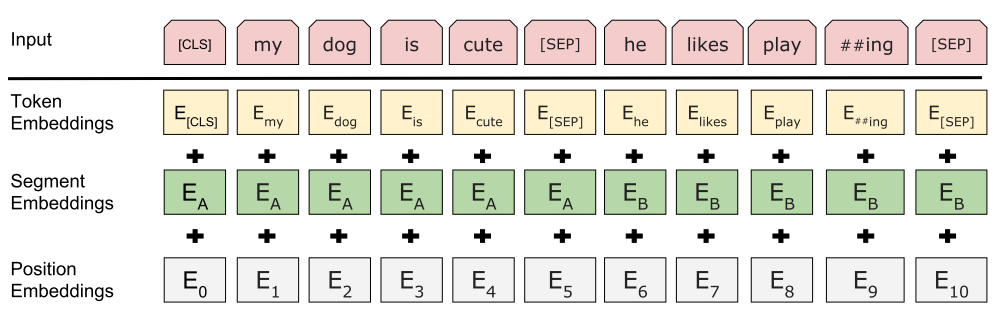
\includegraphics[width=\linewidth]{img/bert-input.png}	
	\end{figure}
	
\end{frame}


\subsection{Pre-training}


\begin{frame}{BERT: Self-supervised multi-task pre-training}
	
	Prepare two auxiliary tasks that need no labeled data
	
	\bigskip
	
	\begin{columns}
		\begin{column}{0.5\linewidth}
			\begin{small}
				Task 1: Cloze-test task
				\begin{itemize}
					\item 	Predict the masked WordPiece unit (multi-class, 30k classes)
				\end{itemize}
				
				
				Task 2: Consecutive segment prediction
				
				\begin{itemize}
					\item Did the second text segment appeared after the first segment? (binary)
				\end{itemize}
			\end{small}
			
		\end{column}
		\begin{column}{0.5\linewidth}
			
			\begin{figure}
				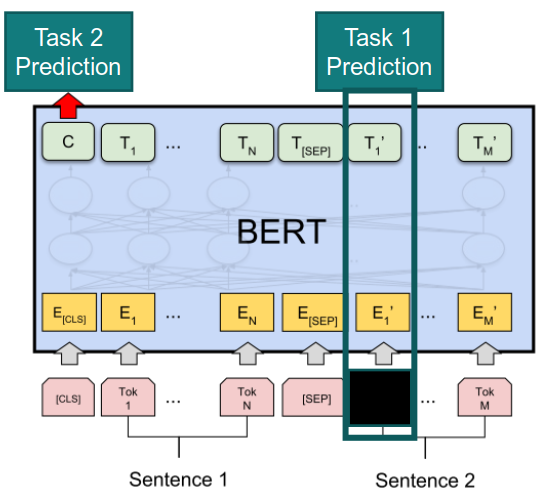
\includegraphics[width=\linewidth]{img/bert-pretraining.png}
			\end{figure}
		\end{column}
		
	\end{columns}
\end{frame}




\begin{frame}{BERT: Pre-training data generation}
	
	Take the entire Wikipedia (in 100 languages; 2,5 billion words)
	
	To generate a single training instance, sample two segments (max combined length 512 WordPiece tokens)
	
	\begin{itemize}
		\item For Task 2, replace the second segment randomly in 50\% (negative samples)
		\item For Task 1, choose random 15\% of the tokens, and in 80\% replace with a [MASK] 
	\end{itemize}
	
	
\end{frame}


\begin{frame}{BERT: Pre-training data -- Simplified example}
	
	\begin{columns}
		\begin{column}{0.5\linewidth}
			\begin{figure}
				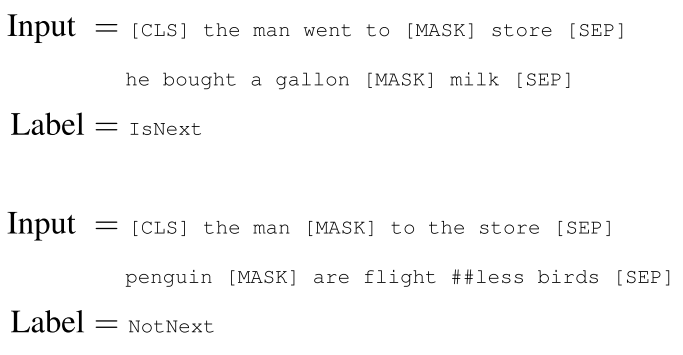
\includegraphics[width=\linewidth]{img/bert-pretraining2.png}
			\end{figure}
		\end{column}
		\begin{column}{0.5\linewidth}
			\begin{small}
				
				\begin{itemize}
					\item $<$PAD$>$ding is missing
					\item The actual segments are longer and not necessarily actual sentences (just spans)
					\item The WordPiece tokens match full words / morphology well in this English text, but recall the ones we have seen before
				\end{itemize}
			\end{small}
		\end{column}
	\end{columns}
	
	
\end{frame}



\subsection{Downstream tasks and fine-tuning}

\begin{frame}{BERT: Representing various NLP tasks}
	
	\begin{figure}
		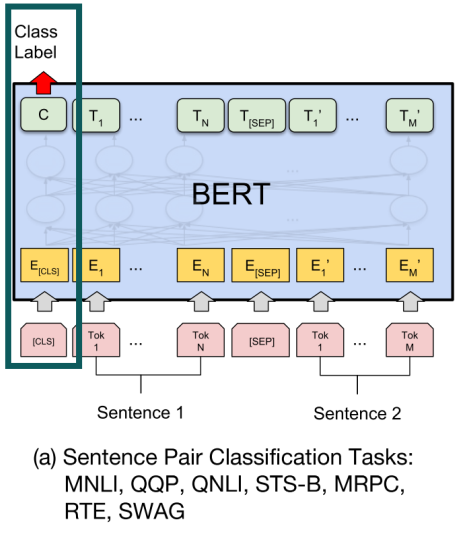
\includegraphics[width=0.5\linewidth]{img/task1.png}
	\end{figure}
	
	That explains the special [CLS] token at sequence start
	
\end{frame}



\begin{frame}{BERT: Representing various NLP tasks}
	
	\begin{figure}
		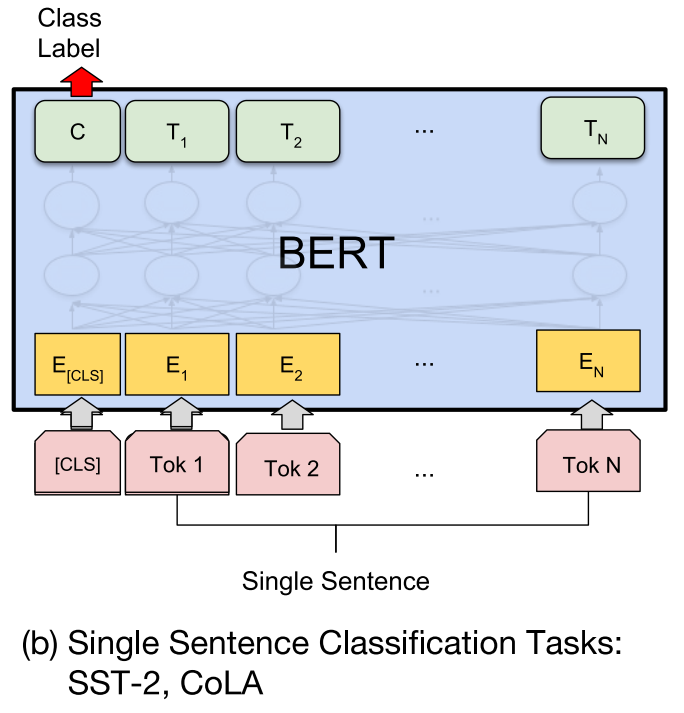
\includegraphics[width=0.6\linewidth]{img/task2.png}
	\end{figure}
	
	
\end{frame}



\begin{frame}{BERT: Representing various NLP tasks}
	
	\begin{figure}
		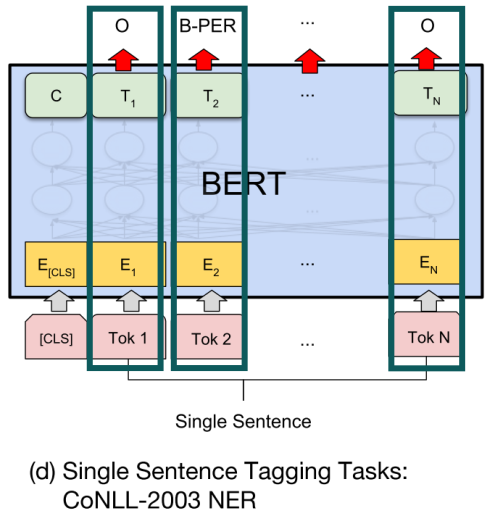
\includegraphics[width=0.5\linewidth]{img/task3.png}
	\end{figure}
	
	
	Not conditioned on surrounding predictions	
	
\end{frame}

\begin{frame}{BERT: Very abstract view}
	
	\begin{figure}
		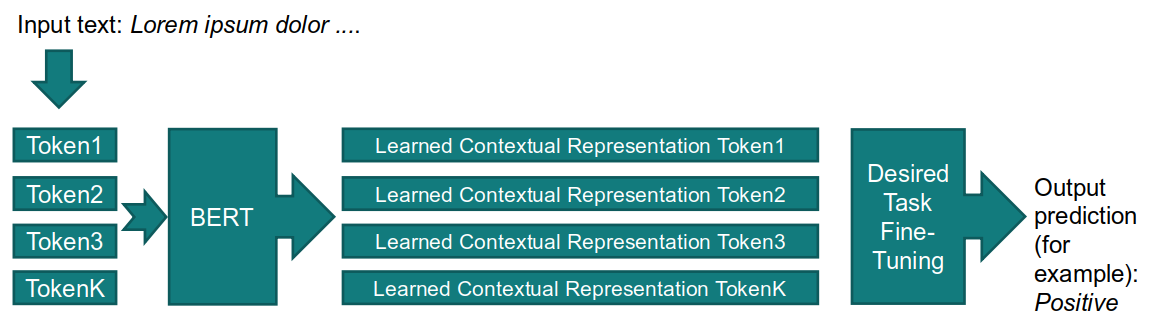
\includegraphics[width=\linewidth]{img/bert1.png}
	\end{figure}	
	
\end{frame}


\begin{frame}{BERT: Very abstract view}
	
	\begin{figure}
		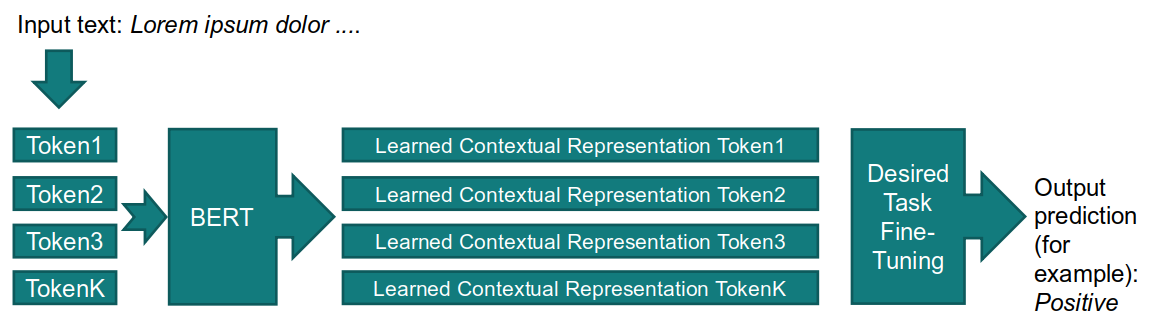
\includegraphics[width=\linewidth]{img/bert1.png}
	\end{figure}	
	
	Pretraining BERT took originally 4 days on 64 TPUs\footnote{Can be done more efficiently, see, e.g., \citet{izsak-etal-2021-train}}
	
	\bigskip
	
	Once pre-trained, transfer and "fine-tune" on your small-data task and get competitive results


	
\begin{tikzpicture}[overlay, remember picture] 
	\node at (current page.north east)[ref] {\fullcite{izsak-etal-2021-train} \par};
\end{tikzpicture}

	
\end{frame}


\begin{frame}{Recap}
	
	BERT stays on the shoulders of many clever concepts and techniques, mastered into a single model
	
\textbf{What do we know about how BERT works?}

	
\emph{``BERTology has clearly come a long way, but it is fair to say we still have more questions than answers about how BERT works.''} --- \citet{Rogers.et.al.2020.BERT}\footnote{Highly recommended reading!}
	
	
\begin{tikzpicture}[overlay, remember picture] 
	\node at (current page.north east)[ref] {\fullcite{Rogers.et.al.2020.BERT} \par};
\end{tikzpicture}
	
\end{frame}





\begin{frame}{License and credits}

	\begin{columns}
		\begin{column}{0.7\textwidth}
			Licensed under Creative Commons Attribution-ShareAlike 4.0 International (CC BY-SA 4.0)
		\end{column}
		\begin{column}{0.2\textwidth}
			
\includegraphics[width=0.9\linewidth]{img/cc-by-sa-icon.pdf}
		\end{column}
	\end{columns}
	
	\bigskip
	
	Credits
	
	\begin{scriptsize}
		
		Ivan Habernal
		
		Content from ACL Anthology papers licensed under CC-BY \url{https://www.aclweb.org/anthology}
		
	
	\end{scriptsize}
	
\end{frame}



\end{document}

